\section{Background}\label{sec:background}

\begin{figure}
    \centering
    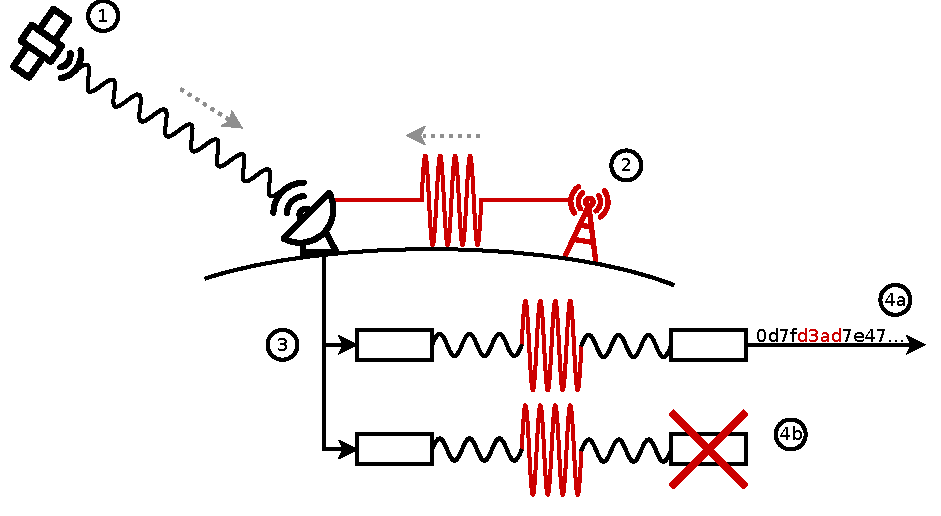
\includegraphics[width=\columnwidth]{diagrams/attack_illustration.pdf}
    \caption{A demonstration of signal injection through overshadowing on a satellite downlink, resulting in the decoding of arbitrary bytes.}
    \label{fig:attack-illustration}
\end{figure}

\textbf{TODO figure out where to put this figure}

% TODO: add info about Google Maps
\begin{table*}
    \resizebox{\textwidth}{!}{%
    \begin{tabular}{lllll}
        \toprule
                     &       & \multicolumn{2}{c}{Satellites} & \\
        \cmidrule(lr){3-4}
        Organization & Usage & Provider & Nature & Data Access \\
        \midrule
        Planet Labs~\cite{planetProducts} & Various (intelligence, infrastructure, & Planet Labs & Self-operated & Commercial \\
                    & land use, water use) & & & \\
        Global Forest Watch~\cite{gfwMap} & Forest monitoring, carbon use, deforestation & Planet Labs & Commercial & Open access \\
        California Forest Observatory~\cite{cfoMap} & Monitoring forest fires in California & Planet Labs & Commercial & Open access \\
        ESRI~\cite{esriMap} & Land-use and land-cover maps & ESA (Sentinel-2) & Open access & Open access \\
        %Salo Sciences (TODO only bring back if I can say something about "forest restoration monitoring" project) & Conservation, climate monitoring & Planet Labs & Commercial & \\
        Meta~\cite{metaMap} & Population density maps & DigitalGlobe & Commercial & Open access \\
        Cloud to Street~\cite{cloudToStreet} & Flood tracking (disasters and insurance) & NASA (Terra/Aqua) & Open access & Commercial \\
        NCX Basemap~\cite{ncxBasemap} & Timber and carbon value monitoring in the USA & NASA & Open access & Commercial \\
        Upstream Tech HydroForecast~\cite{hydroforecast} & Water flow and weather intelligence & NASA (Terra/Aqua) & Open access & Commercial \\
        NASA FIRMS~\cite{nasaFirms} & Fire detection and management & NASA (EOS) & Self-operated & Open access \\
        \bottomrule
    \end{tabular}%
    }
    \caption{Information on a number of satellite-derived datasets, including the satellite providers used to source the data.}
    \label{tab:satellite-derived-datasets}
\end{table*}

Satellite data has become crucial to a wide range of both public and private organizations.
It is now possible to access near real time high-resolution images of the Earth, updating within hours or less of the initial readings being taken, in addition to infrared and other sensor readings.
Building upon this raw data, a growing market for \textit{satellite-derived datasets} has emerged: data which has been produced by processing and analysing the raw satellite data for a wide variety of use cases. % TODO: mention satellite-derived datasets throughout the paper since we introduce the term here
These include critical national infrastructure such as forest fire and storm detection, and research-oriented purposes such as land and water management.
End users may be more familiar with systems such as Google Maps, which provides a fire overlay and reroutes drivers around currently active fires and smoke zones.

Table~\ref{tab:satellite-derived-datasets} summarises a number of currently available satellite-derived datasets.
These are designed for various uses, and are derived from a mixture of self-operated, commercial, and open access satellites.

The source of the base satellite dataset is chosen based on the organization and use case.
Some businesses operate their own satellite network and then process the data, granting fine-grained control at the cost of having to launch and maintain their own satellites.
For many organizations operating a satellite network is an unnecessary expense; many opt to instead acquire data from other satellite operators.
This data can either be purchased from a private satellite operator, or received from a publicly broadcast satellite such as one from NASA's fleet of Earth Observing System (EOS) satellites.
Signals from the latter can be received by anyone with a compatible ground station \textbf{TODO cite}, providing an immensely useful service to both private and public organizations.

% Availability, representativeness, utilisation by downstream consumers
% Understanding the bounds of the attacker
% How people rely on the data
% Packet-based data downlink protocols that are unencrypted
% Manifold security issues but seemingly little thought, with sizeable impact
% GNSS spoofing -

% https://www.usenix.org/conference/usenixsecurity19/presentation/yang-hojoon

\subsection{Research Applicability}

In this research we demonstrate how implicitly trusting input data opens the gateway for more sophisticated attacks against the processing pipeline through signal injection.
As a case study, we focus on \textit{Terra} and \textit{Aqua}, two open access satellites within NASA's EOS fleet.
Being open access, they are among the best publicly-documented satellite systems, and the data they collect is trusted by a wide range of applications through derived datasetes in both the private and public sectors.
These systems provide no cryptographic authenticity by design, raising concerns about their susceptibility to attack as the barrier to entry for attackers lowers -- in this work we assess the severity of this threat, and how best to mitigate it.

The extent that this research relates to other satellite systems depends upon the design of the communications layer in question, and at which stage, if any, secure cryptographic primitives are used.
This work therefore directly applies to all publicly broadcast satellites, such as other satellites in the EOS fleet and the GOES satellites by NOAA~\textbf{TODO: cite}, which are unencrypted by design for ease of public access. % TODO: document which other satellites are therefore usable
However, satellites which apply sound cryptographic mechanisms such as \textit{Space Data Link Security} (SDLS) to sign or encrypt at the data link layer, using good key and subkey management schemes to protect against leaks, and checksums to verify integrity, are resilient to these manipulations.

% TODO: insert diagram of common space comms protocols

% TODO: find out which other satellites are unencrypted, and especially those which are new and use CCSDS
% Are they generally encrypted above the CCSDS layer?

Despite this, there are similar techniques which can affect even satellites with encrypted communications if improperly implemented.
Where encryption is left only for the network layer or above in the protocol stack, attackers can manipulate the low-level protocol headers and data to trigger potential vulnerabilities in the decoding software.
Alongside these issues, vulnerabilities in the decoding software are prevalent and pose a real danger to not only the trustworthiness of the processed data but the processing system itself.
% This is often because decoders are written to only handle the subset of any given specification that their satellite uses under nominal conditions, failing under unexpected circumstances.
% Other times, this is because the overall decoding system has slowly accumulated technical deficiencies, as one team tries to hack around not quite understanding the existing software.
We justify this claim in Section~\textbf{TODO} through a security audit of NASA's flagship \textit{International Planetary Observation Processing Package} (IPOPP) software distribution.

Also, where cryptographic key management has been poor, keys can often be leaked or reverse engineered, compromising data confidentiality and potentially rendering the satellite vulnerable to spoofing\footnote{Whether key recovery can result in spoofing depends on the encryption scheme used, and particularly upon whether the keys are symmetric.}.
This is unfortunately common; decryption keys for the Korean satellite GEO-KOMPSAT-2A were leaked from code samples on the Korea Meteorological Administration website, and to this day remain unrevoked and available on their website~\cite{xrit-rx}.
Other satellites implement either poor cryptography, or good cryptography poorly, and can therefore have their keys reversed.
For example, COMS-1 uses single DES~\cite{lrit-key-dec}, with its keys successfully reversed from the satellite data. \textbf{TODO: check this is really how it was done. Subleties in the blog post...}
We should continue to expect that more encrypted satellite communications become publicly decryptable, as once-secure encryption standards and practises cause leaked keys, some of which will be irrevocably baked into the firmware.

% Tasked vs untasked images

\subsection{NASA Earth Observing System}

% One of the data providers
% Loads of people depend on it, but nobody thought of security

Terra and Aqua, as core satellites within the EOS fleet, provide high resolution sensor readings across a variety of detectors.
Images of the Earth's surface can be derived from their on board \textit{Moderate Resolution Imaging Spectroradiometer} (MODIS) sensor, which produce calibrated light readings across frequency bands wider than the visible spectrum.
This allows satellite-derived datasets measuring phenomena such as forest fires, ozone scattering, and surface luminosity to be created.
These can be viewed live from NASA's Worldview, which overlays color-corrected surface images with geographically located satellite derived datasets Figure~\ref{fig:bushfire}.

\begin{figure}
    \centering
    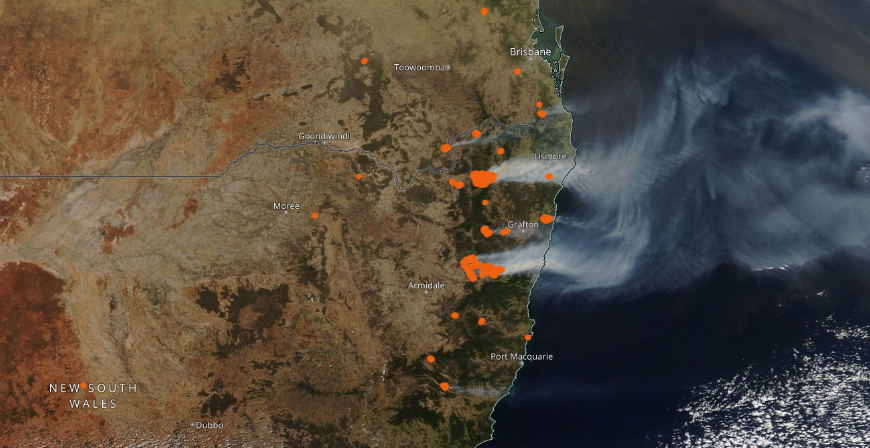
\includegraphics[width=\columnwidth]{diagrams/bushfire.png}
    \caption{The 2019 Australia bushfires as seen from Aqua's MODIS instrument, annotated with the \textit{Fires and Thermal Anomalies} dataset on NASA's worldview.\protect\footnotemark}
    \label{fig:bushfire}
\end{figure}

\footnotetext{Image taken from \url{https://worldview.earthdata.nasa.gov/?v=138.5214305912576,-37.663755528187544,165.90196079866635,-23.47436617591061\&as=2019-09-07-T00\%3A00\%3A00Z\&ae=2019-10-26-T16\%3A00\%3A00Z\&l=MODIS\_Combined\_Thermal\_Anomalies\_All,VIIRS\_SNPP\_Thermal\_Anomalies\_375m\_Day(hidden),VIIRS\_SNPP\_Thermal\_Anomalies\_375m\_Night(hidden),Reference\_Labels\_15m,Reference\_Features\_15m,Coastlines\_15m,VIIRS\_SNPP\_CorrectedReflectance\_TrueColor(hidden),MODIS\_Aqua\_CorrectedReflectance\_TrueColor,MODIS\_Terra\_CorrectedReflectance\_TrueColor(hidden)\&lg=false\&al=true\&av=3.5\&ab=on\&t=2019-09-07-T02\%3A00\%3A00Z}}

Thanks to their opposite polar sun-synchronous orbits, Terra and Aqua together image the entire surface of the Earth twice per day \textbf{TODO: fact check}, which has opened up possibilities for near real time analysis for time-critical applications, such as fire and storm detection.

In addition to buffering and downlinking this data via the TDRSS satellite relay network to NASA in White Sands, New Mexico~\textbf{TODO: cite}, the satellites also continuously broadcast their sensor data via a mode known as direct broadcast.
Therefore, anyone with access to the relevant X-band hardware can receive satellite images from their area with essentially zero latency.
This key design decision, alongside demonstrating true commitment to open access data, is particularly useful for applications where the several hour delay waiting for Terra or Aqua to be within range of a relay satellite is unacceptable. \textbf{TODO: cite}

% TODO: CADU diagram, with all the internals exposed

The data is downlinked in almost exactly the same format for both the main data dump and the direct broadcast.
Packets from the MODIS instrument are encapsulated wthin the CCSDS Space Packet Protocol (SPP), which are packed within an unencrypted custom data link protocol known as the \textit{Channel Access Data Unit}, or CADU.
Finally, the CADUs are modulated using \textit{Quadrature Phase Shift Keying} (QPSK) and transmitted on the X-band, centered at 8160\,MHz. \textbf{TODO: is this the same for both DB and TDRSS dump?}

% TODO: diagram of data levels of processing for IPOPP
The data processing systems run at both the main NASA complex and the direct broadcast ground stations are highly similar, both generally being derived from software found in the open source IPOPP distribution.
This enables the direct broadcast ground stations to generate the same data products, but for their particular area.
Additionally, it provides a backup system by which NASA can recover missing data, if it was successfully received by a different ground station during direct broadcast.
However, the uniformity of the software distribution means that vulnerabilities discovered in the software have a wide impact.

% TODO: is such an in-depth explanation required here?
The raw SPP packet data is known as \textit{Level 0}, and is processed through a chain of programs distributed through the IPOPP framework to generate higher-level satellite-derived datasets.
The other EOS fleet satellites are processed in much the same way.
The Level 0 data is processed into \textit{Level 1}: an easier to use heirarchical data format, optionally geolocated to a subpixel accuracy using timing information, the satellite's orbital parameters, and an accurate model of the Earth's surface.
Level 1 data is processed into a variety of \textit{Level 2} datasets, including fire detection, land surface temperature values, vegetation detection, etc.
Finally, certain Level 3 datasets are produced, which generally consist of composites of the Level 2 data for specific purposes, such as analysing post-fire burned areas.

Data across these various levels is available within minutes of being received by direct broadcast ground stations, but is also distributed centrally by NASA after being downlinked by TDRSS.
Users can download from the main NASA archives from one of several \textit{Distributed Active Archive Centers} (DAACs), which provide datasets going back to the beginning of their respective missions.
This data is intended to be downloaded and processed locally on and end user's machine, but is also periodically reprocessed in bulk as new algorithms become available.

Additionally, there exist several specialised near real time data APIs which are utilised widely in applications such as forest fire incident response~\cite{nasaFirms} and flood detection~\cite{nasaFlood}, where running a custom ground station would be impractical and prohibitively expensive.
Despite being more prone to false positives than the multi-day processed data, the lower latency and entirely automated process makes this option attractive for many applications.

\subsection{Forest Fire Live Alerting Systems}

Fire management and incident response represents one such use case of the MODIS instrument, which has improved the fire response capability of over 90 countries \textbf{TODO: cite}.
Although fire departments have little reason to run their own direct broadcast groundstations, the application is still time-critical.
Therefore, NASA has invested in the Fire Information for Resource Management System (FIRMS)~\cite{firmsIndex}, which provides near real time active fire data, defined to be within three hours of observation.
Among other services, FIRMS provides a fire notification API which will deliver notifications of new and active fires within a requested region, which is used to inform firefighters and coordinate their response.
\textbf{TODO: add information on who uses this service, maybe a table. Does Google Maps use this?}
The data is derived from processing the raw Aqua and Terra data with the programs in IPOPP.

However, despite its importance as trusted infrastructure, FIRMS ultimately relies on unencrypted MODIS data which is therefore vulnerable to signal injection.
Through carefully crafting input data to pass any existing integrity checks in the processing pipeline and overshadowing the X-band radio signal, an attacker has the potential to disrupt the fire detection stages of the pipeline, and therefore anyone who relies upon the data.

We proceed to precisely define the nature of the threat in Section~\ref{sec:threat-model}, and describe how an attacker can exploit FIRMS and other processing pipeline stages in Section~\ref{sec:attack}.
We go on to validate the feasibility of the overshadowing approach in Section~\ref{sec:evaluation}, including the capabilities that the attacker requires to be successful.


\subsection{Related Work}

\textbf{TODO write}
\begin{itemize}
    \item existing work in signal sniffing/spoofing, ads-b?
    \item existing work in satellite security?
    \item explain how our work is novel and builds on these
\end{itemize}

Our work builds on \textbf{TODO}

Existing work has shown that it is possible to spoof satellite signals, particularly when not encrypted; \textbf{TODO} demonstrates this using the GPS positioning satellites.
By exploiting the unauthenticated nature of the signals it is possible to modify the unauthenticated data; our work builds on this by demonstrating that this is also possible for satellites for which the receiving and broadcasting equipment was previously thought to make such attacks prohibitively expensive.
We also look beyond the payload and look at attacks on the data processing system itself to create novel attacks.

\textbf{TODO something about packet-based broadcast vs continuous broadcast?}

There is also wider work in the security community surrounding signal spoofing and its detection -- for instance, Čapkun et al.\ detect GPS spoofing by observing the physical properties of the signal alongside inspecting downlinked data \textbf{TODO cite SPREE}.
\textbf{TODO more?}
We \textbf{TODO}.
